\section{Verwitterung}
\begin{myExBox}[title=Verwitterung]
\textbf{Prozesse} der Lockerung, Aufbereitung und Zerstörung von Gesteinen sowie Mineralien an oder nahe der Erdoberfläche durch die Einwirkung \textbf{physikalischer} (mechanischer), \textbf{chemischer} oder \textbf{biogener} Einflüsse. Die Stärke der Verwitterung hängt ab vom Klima, den Eigenschaften des Gesteins sowie der Zeitdauer, während dem die Prozesse dauern.
\end{myExBox}

\notiz{5}

\begin{table}[H]
\centering
\begin{tabular}{@{}p{5cm}||p{8cm}|p{3cm}@{}}
\toprule
\textbf{Verwitterungstyp} & \textbf{Beschreibung und Beispiele} & \textbf{Produkt} \\
\midrule\midrule
\textbf{Temperaturverwitterung} & Temperaturschwankungen durch Sonneneinstrahlung: Erwärmung (Ausdehnung) am Tag, Abkühlung (Schrumpfung) in der Nacht erzeugen Spannungen. & Körnig-eckiger Gesteinsschutt \\\midrule
\textbf{Frostverwitterung} & Volumenvergrösserung von gefrierendem Wasser (um 9 \%) erzeugt Druck. & Blöcke \\\midrule
\textbf{Salzverwitterung} & Verdunstung von Wasser, Kristallisation der gelösten Salze. Ausdehnung durch Kristallisationsdruck führt zu Sprengung. & Rundliche Hohlräume \\\midrule
\textbf{Biologisch-physikalische Verwitterung} & Sprengung durch Pflanzenwurzeln. & Blöcke \\\midrule
\bottomrule
\end{tabular}
\caption{\textbf{Physikalische Verwitterung: Typen und Prozesse}}
\end{table}

\begin{table}[H]
\centering
\begin{tabular}{@{}p{5cm}||p{8cm}|p{3cm}@{}}
\toprule
\textbf{Verwitterungstyp} & \textbf{Beschreibung und Beispiele} & \textbf{Produkt} \\
\midrule\midrule
\textbf{Lösungsverwitterung} & Lösen von Substanzen in Wasser, z.B. Steinsalz, Kalk, Gips. \newline Sonderformen: \textbf{Kohlensäureverwitterung}, Rauchgasverwitterung. & Hartes Wasser \\\midrule
\textbf{Oxidationsverwitterung} & Oxidation von z.B. Eisen mit Sauerstoff in Luft und/oder Wasser. & Rost \\\midrule
\textbf{Hydrationsverwitterung} & Volumenvergrösserung durch Anlagerung von Wassermolekülen im Kristallgitter von Mineralien. & Zerfallene Mineralien \\\midrule
\textbf{Biologisch-chemische Verwitterung} & Organische Säuren von Pflanzen lösen Mineralien auf. & Humus \\\midrule

\end{tabular}
\caption{\textbf{Chemische Verwitterung: Typen und Prozesse}}
\end{table}

\section{Erosion}
\begin{myExBox}[title=Abtragung]
Durch Wasser (Flusserosion), Wind (Winderosion oder Deflation) und Eis (Gletschererosion), jedoch auch unmittelbar durch die Schwerkraft (z.B. Bergsturz) wird das aufbereitete Gesteinsmaterial verlagert. Eine linienhafte Abtragung (z.B. Flüsse) wird als \textbf{Erosion}, eine eher flächenhafte hingegen als \textbf{Denudation} bezeichnet.
\end{myExBox}
\notiz{5}
\begin{myExBox}[title=Ablagerung]
Nach dem Transport durch Wasser, Wind und Eis werden die festen Stoffe an bestimmten Orten wieder abgesetzt oder ausgeschieden, was man allgemein als Ablagerung, Akkumulation oder Sedimentation bezeichnet. Dabei unterscheidet man zwischen klastischen (z.B. Sand), chemischen (z.B. Gips) und biogenen Sedimenten (z.B. Korallenriff)
\end{myExBox}
\notiz{5}

\begin{myexercise}[(Quelle: \cite{hep})]
Die Alpen heben sich seit circa 30 Millionen Jahren um durchschnittlich 0.5 bis 1 mm pro Jahr. Damit sollten die höchsten Berggipfel heute eigentlich 15'000 bis 30'000 m hoch sein.

Wieso erreichen die Alpen ``nur'' circa 4000 m Höhe?
\begin{figure}[H]
\centering
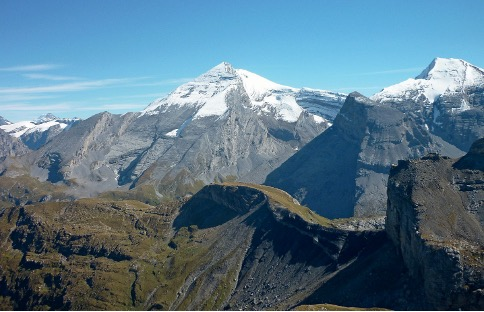
\includegraphics[width=0.7\linewidth]{Private/Images/Altels}
\caption{Der Altels im Berner Oberland, 3629 m ü. M. (© Fritz Lauber).}
\label{fig:altels}
\end{figure}
\end{myexercise}

\begin{myexercise}
Nennen Sie die Verwitterungsformen, welche man in der Schweiz antreffen kann. Begründen Sie Ihre Antwort.
\end{myexercise}